\section{Introduction of the Continuous and Proactive Security Assessment Model (CAPSAM)}

\section{Theoretical Foundations of CAPSAM}
    \subsection{Agile Methodologies}

    \subsection{DevSecOps Principles}

\section{The Five Pillars of CAPSAM}

    \subsection{Continuous Risk Assessment}

    \subsection{Proactive Mitigation Strategies}

    \subsection{Incident Response Planning}

    \subsection{Regular Audits and Reviews}

    \subsection{Feedback Loop}

\section{CAPSAM Cycle for Integration with Agile and DevSecOps}
\begin{figure}[htbp]
    \centering
    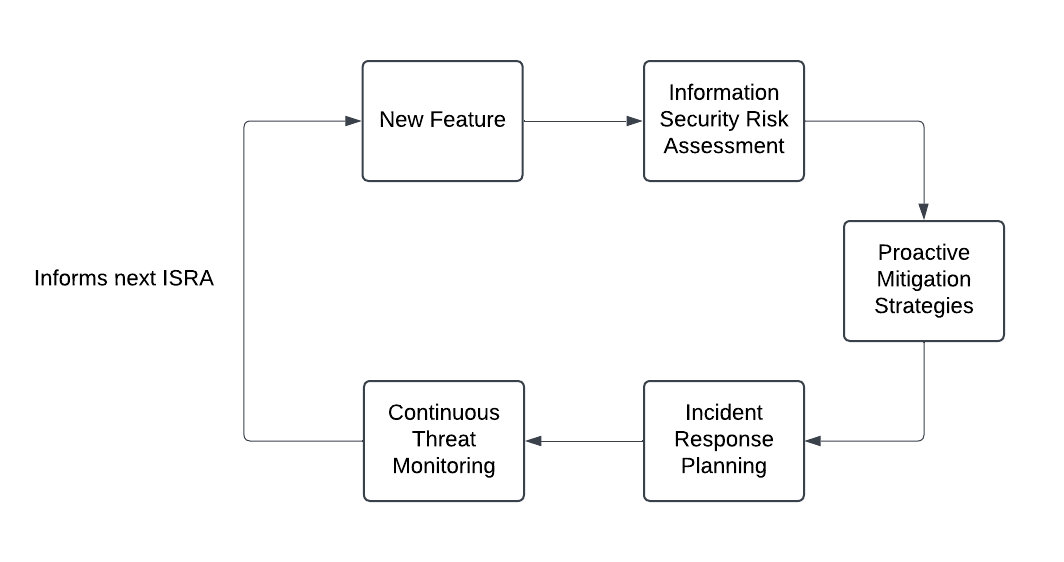
\includegraphics[width=0.8\textwidth]{figures/CAPSAM-Cycle.png}
    \caption{CAPSAM Cycle for Integrating Security into New Feature Development, Highlighting Continuous Risk Assessment, Proactive Mitigation, and Feedback Loops in Agile and DevSecOps Environments.}
    \label{fig:CAPSAM}
\end{figure}

\subsection{Agile Integration of CAPSAM}

\subsection{DevSecOps Culture and TMT Involvement}

\subsection{Where TMT Fits in the CAPSAM Cycle}

\section{CAPSAM as a Strategic Approach}

\section{Benefits of CAPSAM Over Reactive Approaches}
